\documentclass{report}

% настройки для титульного листа
\newcommand{\kafedranum}{} %кафедра
\newcommand{\kafedraname}{} %название кафедры
\newcommand{\prepodname}{} %имя препода
\newcommand{\discname}{} %дисциплина
\newcommand{\themename}{} %номер КДЗ
\newcommand{\coursenum}{} %номер курса
\newcommand{\groupname}{} %группа
\newcommand{\speciality}{} %специальность
\newcommand{\fio}{} %ФИО%

\usepackage[T1]{fontenc}
\usepackage{fontspec}
\usepackage{graphicx}
\usepackage{indentfirst}
\usepackage[T2A,T1]{fontenc}
\usepackage[utf8]{inputenc}
\usepackage[russian]{babel}
\usepackage{hyphenat}
\usepackage{hyperref}
\usepackage{tocloft}
\usepackage{csquotes}
\usepackage{amsmath}
\usepackage{sectsty}
\usepackage{pdfpages}
\setmainfont{Times New Roman}
\usepackage[fontsize=14pt]{fontsize}
\setlength{\parskip}{0pt}

\sectionfont{\fontsize{14}{14}\selectfont}
\subsectionfont{\fontsize{14}{14}\selectfont}
\linespread{1.5}
\setlength{\parindent}{1.25cm}

 
\hypersetup{ 
     colorlinks=true, 
     linkcolor=black, 
     filecolor=blue, 
     citecolor = black,       
     urlcolor=blue, 
     }

\BeforeBeginEnvironment{verbatim}{\def\baselinestretch{1}}
\setmonofont[Scale=0.85]{Courier New}
\setlength{\cftsecindent}{0pt}
\setlength{\cftsubsecindent}{0pt}

\usepackage[a4paper, left=30mm,top=20mm,bottom=20mm,right=10mm]{geometry}

\newcommand{\intro}{%
  \section*{Введение}
  \addcontentsline{toc}{section}{Введение}
}

\newcommand{\conclusion}{%
  \section*{Заключение}
  \addcontentsline{toc}{section}{Заключение}
}

\renewcommand{\cftbeforetoctitleskip}{0cm}
\cftsetindents{section}{0em}{2em}
\cftsetindents{subsection}{0em}{2em}
\renewcommand{\cfttoctitlefont}{\normalfont\bfseries}
\renewcommand{\cftaftertoctitleskip}{0.0\baselineskip}
\renewcommand{\cftsecleader}{\cftdotfill{\cftdotsep}}
\renewcommand{\cftsubsecleader}{\cftdotfill{\cftdotsep}}
\renewcommand{\cftdot}{.}
\newcounter{imgcount}

\usepackage{caption}
\DeclareCaptionLabelFormat{mylabel}{Рисунок #2}
\captionsetup{labelformat=mylabel}

\newcommand{\image}[2]{%
  \begin{figure}[htbp]
    \centering
    \includegraphics[width=\textwidth,keepaspectratio]{#1}
    \caption{#2}
    \label{fig:#1}
  \end{figure}
}

\graphicspath{ {./media/}



\begin{document}

% титульник


\begingroup
\fontsize{12}{12}\selectfont
\linespread{1}
\begin{center}

\includegraphics[scale=0.4]{./title/title.png}
\vspace{1em}\\
МИНОБРНАУКИ РОССИИ\\
Федеральное государственное бюджетное образовательное учреждение\\
высшего образования\\
\textbf{«МИРЭА -- Российский технологический университет»}\\
\vspace{1em}
\fontsize{14}{14}\selectfont
\textbf{РТУ МИРЭА}\\
\noindent\rule{16cm}{2pt}
\end{center}
\endgroup

\begin {center}
\blankLine{(название института, филиала)}{Институт кибербезопасности и цифровых технологий}
\blankLine{(наименование кафедры)}{Кафедра КБ-\kafedranum \space \enquote{\kafedraname}}
\end {center}

\begin{center}

\textbf{ОТЧЁТ ПО ЛАБОРАТОРНОЙ РАБОТЕ № \worknum \hspace{4pt}}

\textbf{\MakeUppercase{\workname}}

\textbf{По дисциплине}

\textbf{«\discname»}     

\end {center}
\vspace{1.5em}
\resizebox{\textwidth}{!}{%
\begin{tabular}{lcc}    
Отчёт представлен к\\ рассмотрению: &                      &                                 \\
Студент группы \groupname        & \enquote{\_\_} \_\_\_\_ \the\year{} г. & \underline{\fio}                    \\
                                    &                      & \small(подпись и расшифровка подписи) \\
                                    &                      &                                 \\
Руководитель практики\\ от кафедры: & \enquote{\_\_} \_\_\_\_ \the\year{} г. & \underline{\prepodname}                   \\
                                    &                      & \small(подпись и расшифровка подписи)
\end{tabular}
}
\vfill
\begin{center}
Москва \the\year{}\\
\end{center}

\thispagestyle{empty}
\newpage

 
%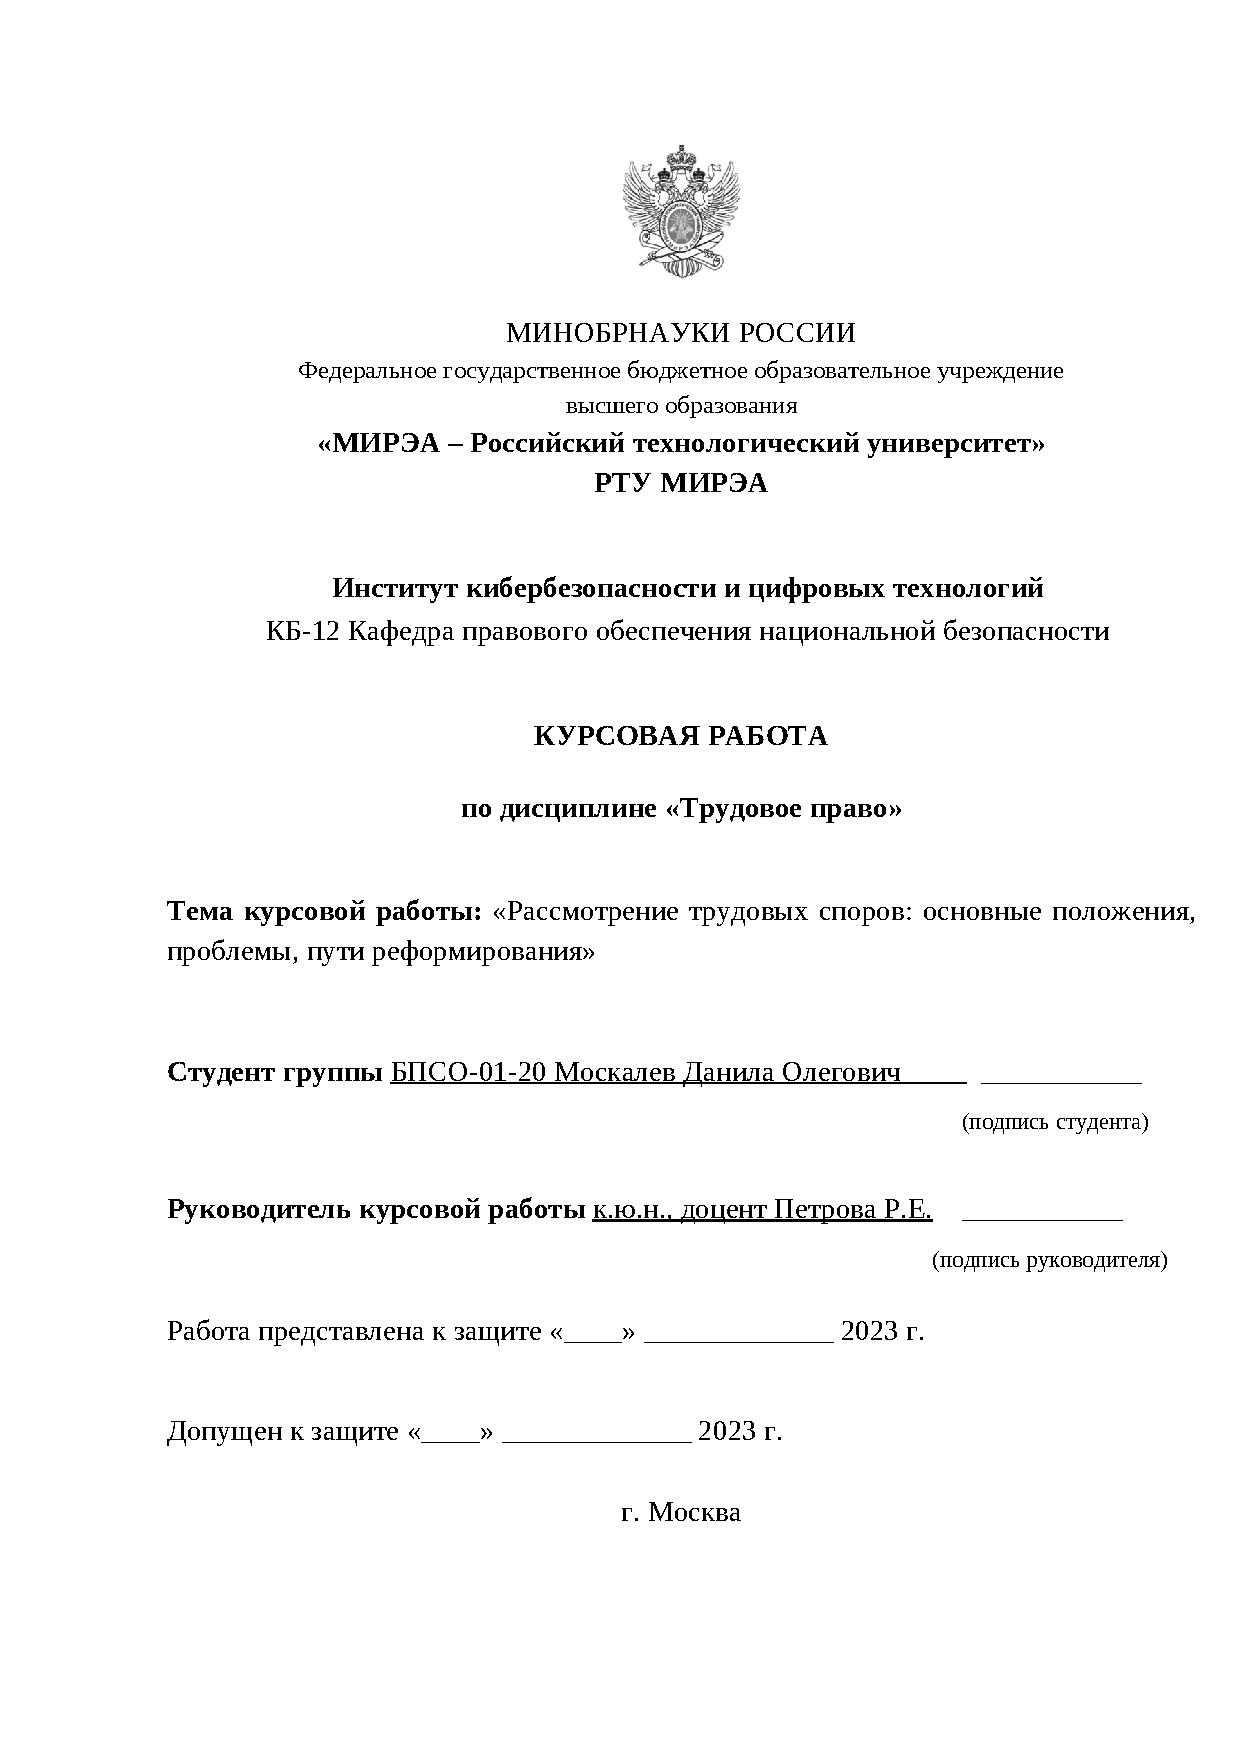
\includepdf{title.pdf} % раскомментить, если титульник дан в формате pdf

%содержание
%Содержание
\newpage
\tableofcontents
\newpage
%Конец содержания


% текст работы
\intro
Здесь идёт красная строка с отступом в 1,5 см. Шрифт – Times New Roman 14, обычное начертание. Поля (3 см слева, 2 справа, сверху и снизу по 2) соблюдены.

Межстрочный интервал – полуторный. Интервалы перед и после абзацев отсутствуют, как и отступы слева и справа. Размер бумаги – A4 (210x297 мм). Выравнивание – по ширине. Ориентация – книжная. Цвет текста – чёрный. Положение переплёта – слева.
\newpage

\section{Текст}
\subsection{Текст с рисунком}
Для запуска программы требуется современный компьютер, совместимый с инструкциями SSE2 и с технологией DirectX 9.0c. Подобный компьютер изображён на рисунке 1 -- Компьютер.

\image{computer.png}{Компьютер}

После рисунка идёт интервал в одну строку. Если рисунков в работе много, их следует помещать в приложении. Подписи должны быть лаконичными.

\newpage
\conclusion

Lorem ipsum dolor sit amet, consectetur adipiscing elit, sed do eiusmod tempor incididunt ut labore et dolore magna aliqua. Ut enim ad minim veniam, quis nostrud exercitation ullamco laboris nisi ut aliquip ex ea commodo consequat. Duis aute irure dolor in reprehenderit in voluptate velit esse cillum dolore eu fugiat nulla pariatur. Excepteur sint occaecat cupidatat non proident, sunt in culpa qui officia deserunt mollit anim id est laborum.


% код
\newpage
\chapter*{Исходный код программы}
\addcontentsline{toc}{chapter}{Исходный код программы}

\begin{verbatim}

\end{verbatim}


\end{document}
